\problem{Podziały drzew} %B-3

\subproblem %B-3(a)
Fakt oczywiście zachodzi dla drzew o~co najwyżej trzech węzłach, dlatego w~dalszej części dowodu założymy, że $n\ge4$.
Rozważmy ciąg węzłów $\langle x_0,x_1,\dots,x_k\rangle$, w~którym $x_0$ jest korzeniem, $x_k$ jest liściem, a~dla $i=1$, 2, \dots, $k$, $x_i$ jest korzeniem poddrzewa węzła $x_{i-1}$ o~większym rozmiarze (w~przypadku, gdy lewe i~prawe poddrzewo $x_{i-1}$ są tego samego rozmiaru, $x_i$ jest korzeniem dowolnego z~nich).
Oznaczmy przez $s(x)$ rozmiar poddrzewa o~korzeniu w~$x$.
Dla każdego $i=0$, 1, \dots, $k-1$ zachodzi $s(x_i)\le2s(x_{i+1})+1$.
Oczywiście ciąg $\langle s(x_0),s(x_1),\dots,s(x_k)\rangle$ maleje od $n$ do 1, dlatego musi istnieć takie $j$, że $s(x_j)>n/4$ i~$s(x_{j+1})\le n/4$.
Zatem usuwając krawędź $\{x_{j-1},x_j\}$, dzielimy węzły drzewa na dwa rozłączne zbiory o~rozmiarach $s(x_j)\le2n/4+1\le3n/4$ oraz $n-s(x_j)<n-n/4=3n/4$.

\subproblem %B-3(b)
Stała $3/4$ jest wystarczająca do dokonywania zrównoważonych podziałów, jak to wykazaliśmy w~punkcie (a).
Przykład drzewa binarnego z~rys.\ \ref{fig:B-3b} pokazuje, że nie można przyjąć na jej miejsce mniejszej wartości.
Usuwając dowolną krawędź tego drzewa, dzielimy zbiór jego wierzchołków na podzbiory, z~których jeden ma trzy elementy.
\begin{figure}[!ht]
	\centering 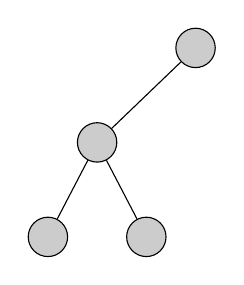
\begin{tikzpicture}[
	level/.style = {level distance=12mm, sibling distance=50mm/2^#1},
	every node/.style = {align=center, inner sep=-1pt, minimum size=5mm, circle, draw, fill=black!20},
]
\node {}
	child {node {}
		child {node {}}
		child {node {}}
	}
	child[missing];
\end{tikzpicture}

	\caption{Drzewo binarne, w~którym najbardziej zrównoważony podział tworzy podzbiór zawierający 3 wierzchołki.} \label{fig:B-3b}
\end{figure}

\subproblem %B-3(c)
Rozważmy następującą procedurę podziału zbioru wierzchołków.
Na początku przyjmujemy, że wynikowe zbiory $A$ i~$B$ są puste.
Usuwając jedną krawędź, możemy podzielić $n$\nbhyphen elementowy zbiór wierzchołków drzewa na dwa podzbiory, z~których większy będzie składać się z~co najwyżej $3n/4$ wierzchołków, co wynika na podstawie punktu (a).
Mniejszy podzbiór sumujemy z~jednym ze zbiorów wynikowych, natomiast większy z~nich będzie podlegał dalszemu podziałowi.
Podczas działania procedury pilnujemy, aby rozmiary zbiorów $A$ i~$B$ nie przekroczyły $\lceil n/2\rceil$.
Procedurę podziału zakończymy w~momencie, gdy jeden z~tych zbiorów będzie zawierał $\lceil n/2\rceil$ elementów, gdyż drugi zbiór zawiera wtedy $\lfloor n/2\rfloor$ elementów.

Zauważmy, że maksymalną liczbę podziałów dla zadanego drzewa wykonamy w~przypadku, gdy po każdym kroku zostanie do podziału zbiór o~rozmiarze $3/4$ rozmiaru zbioru z~poprzedniego kroku.
Niech $k$ będzie taką maksymalną liczbą podziałów drzewa o~$n$ wierzchołkach.
Zachodzi wtedy $(3/4)^kn=1$, ponieważ zbioru jednoelementowego nie trzeba już dalej dzielić.
Stąd mamy $k=\log_{4/3}n$, a~zatem należy usunąć co najwyżej $k=O(\lg n)$ krawędzi.
